\documentclass[10pt,a4paper]{report} 
% Style
\usepackage{amsfonts}
\usepackage{amsmath}
\usepackage{amssymb}
\usepackage[utf8]{inputenc}
\usepackage[T1]{fontenc}
\usepackage[english]{babel}
\usepackage{lmodern} 
\usepackage{graphicx}
\usepackage{color}
\usepackage{float}
\usepackage{url}
\usepackage[numbered]{mcode}

\lstset{extendedchars=\true}
\lstset{inputencoding=ansinew}



% ---Dokumen start---
\begin{document}



% ---Title page ---
\title{Localisation using microphone network\\Sensor fusion -- TSRT14}
\author{Group 12}
\maketitle

\abstract{This is a report for one of the laboration assignments in the course Sensor fusion (TSRT14) at LiTH.
  It consists of estimation, tracking and location for a robot that is moving in a acoustic sensor network.
Several different algorithms are used and compared to each other.}

% ---Innehållsförteckning---
\tableofcontents

\newpage
\chapter{Data gathering}
\label{Data gathering}
The data that is used in this report was gathered during a session at Laboteket.
The setup was a robot that followed a path around a track that was about one meter in diameter.
As the robot went around the track it emitted a pulse two times per second.
The sensors that were used were 7 microphones, that could be placed anywhere around the track.
Three datasets were collected.
First a calibration set. This was collected by placing all the microphones on the same distant from the robot.
This was achived by placing all the microphones on a small segement of a circle with the robot in the center.
The robot was then setup to just emit the pulses and stay still. The setup is displayed in figure \ref{calibtration_setup} below.
\begin{figure}[H]
\begin{center}
  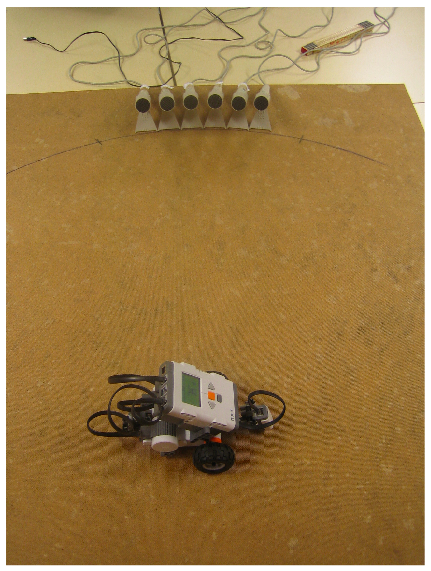
\includegraphics[width = 100pt]{calibration_setup.png}
  \caption{Calibration setup}
  \label{calibtration_setup}
  \end{center}
\end{figure}

After this was done the robot was set up to drive around the track while the microphones recorded data.
Two different setup were used. The placement of the microphones can be seen in Figure \ref{good_setup} and \ref{bad_setup}.
The first setup up was chosen to have microphones spread as even as possible around the track.
This will make the arrival times at the microphones as different as possible.
In the second setup the microphones are closer together and there should be less difference between the arrival time of different microphones.

The robot went around the track about two times for each recording session.
The recorded sound was then processed to find the arrival times for each pulse on every microphone.
These arrival times are then used for tracking and localisation.

The processing of the recordings are done by correlating the recorded signal with the pulse that was transmitted from the robot.
This will give large peaks where the pulses were recorded.

\begin{figure}[!h]
  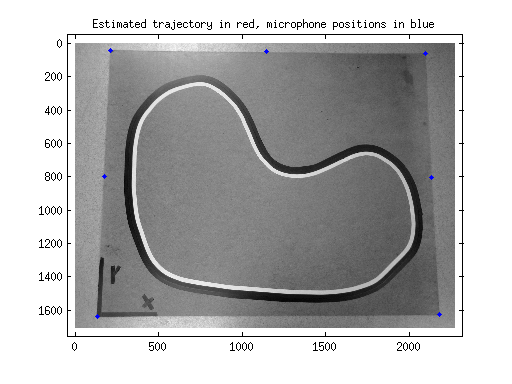
\includegraphics[scale=0.9]{microphone_pos_good.png}
  \caption{Microphone setup one.}
  \label{good_setup}
\end{figure}

\begin{figure}[!h]
  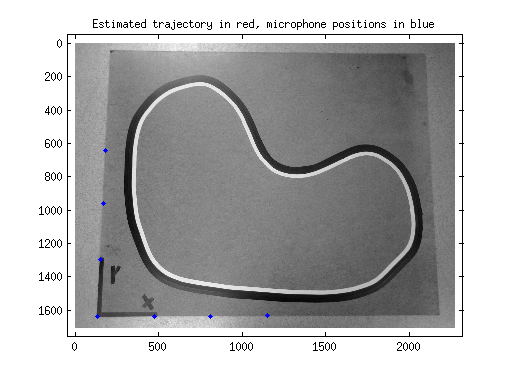
\includegraphics[scale=0.9]{microphone_pos_bad.png}
  \caption{Microphone setup two.}
  \label{bad_setup}
\end{figure}

\newpage
\chapter{Tasks}
\label{Tasks}
The laboration assignment consisted of several task that needed to be completed. This is a description of how they were completed.

\section{Calibration}
\label{Calibration}
The calibration setup described in chapter \ref{Data gathering} in figure \ref{calibtration_setup} produced data which contained the arrival time at each time instant for each sensor. To determine the accuracy of the measurement, the bias and standard deviation is needed. First the error is calculated. Example code for one sensor is shown in the following matlab code. 
\begin{verbatim}
e = tphat(:,1) - mean(tphat, 2);
\end{verbatim}
The same has to be done for the other 6 sensors. The meaning of this is that the mean of the seven sensors at one time instant should be close to the actual value of the arrival time. Since they are placed at en equal distance the arrival time should be the same, but since they are not, we need to compare the measurements to the mean of the sensors, which produces the error.

To compare the empirical probability density function of the measurement noise with a pdfclass distribution, we need to compute a normalized histogram first. This can be achieved using the following code.
\begin{verbatim}
bias = [];
std_deviation = [];
P = [];
mu = [];

figure()
for i = 1:nr_of_sensors
    [N,l] = hist(e(:,i),20);
    Wb = l(2)-l(1); %bin width
    Ny = length(e(:,i)); %nr of samples
    subplot(2,4,i)
    bar(l,N/(Ny*Wb));
    d = i+1;
    title(sprintf( 'Sensor %d', d));
    hold on
    pe_i = ndist(mean(e(:,i)), var(e(:,i)));
    mu = [mu; pe_i.mu];
    P = [P pe_i.P];
    plot(pe_i);
    hold off
    bias = [bias mean(e(:,i))]; % [m] Bias för alla sensorer
    std_deviation = [std_deviation sqrt(var(e(:,i)))];
end
\end{verbatim}
This code also plotts a pdfclass distribution into the same graph for comparison. It also determines the bias and standard deviation for each sensor. 
\begin{figure}[H]
  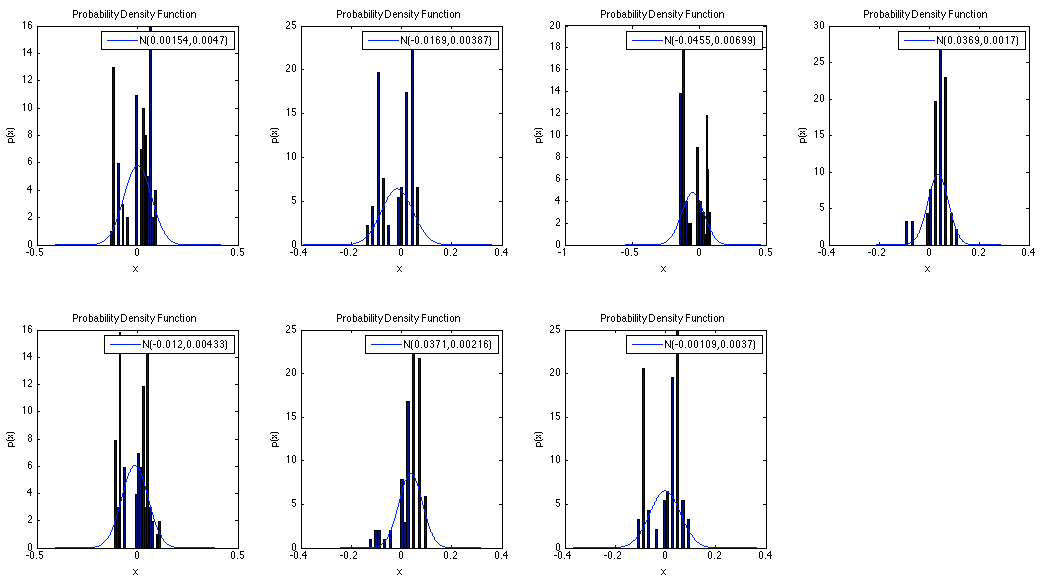
\includegraphics[width = 400pt]{histogram.png}
  \caption{Histogram and pdfclass distribution for each sensor}
  \label{histogram}
\end{figure}
The mean of the standard deviatione is $0.0613$ meters, which can be regarded as the accuracy of the estimation.



\newpage
\section{Sensor modeling}
\label{Sensor modeling}
To do localisation and tracking, a model must be used to process the data in the datasets.
The algorithms used in this laboration need a function that maps the state of the robot to the measurments that has been recorded.
An important observation is that the time when the pulse was emitted from the robot is not known.
This means that either this time has to be estimated as a stat of the robot or that it is eliminated by using the differences of the arrival times in the microphones.
This gives two different sensor models.
In the sensormod toolbox that is used in the course these are reffered to as \emph{TDOA1} and \emph{TDOA2} respectively.
The TDOA1 model can be described using a three dimensional state variabel $x = [p^T, r_0]^T$ 
for the robot and the arrival times of the pulse as a 7-dimensional measurment $y$.
$p = [x1 x2]^T$ is the position of the robot. $r_0$ is the time that the pulse was transmitted from the robot.
The positions of the microphones are denoted $th^i$ where $i$ is the number of the microphone.
The model then becomes
\[
  \bar{y} = 
  \begin{bmatrix}
    |th^1 - p| + r_0 \\ 
    |th^2 - p| + r_0 \\ 
    |th^3 - p| + r_0 \\ 
    |th^4 - p| + r_0 \\ 
    |th^5 - p| + r_0 \\ 
    |th^6 - p| + r_0 \\ 
    |th^7 - p| + r_0 \\ 
  \end{bmatrix} + e
\]
$e$ is the measurment noise. This is estimated in the calibration stage of the asignment.
For simplicity this is assumed to be gaussian and independent.
This sensornetwork can be generated using the \emph{exsensor} funtion from the toolbox.
\begin{verbatim}
exsensor('tdoa1', 3, 1, 2);
\end{verbatim}

The model called TDOA2 uses a two dimensional state $x = p$ with the same $p$ as before.
The differences of the arrival times can then be used to eliminate $r_0$.
There are 7 different microphones wich mean that there are 21 different differences that can be constructed.
In the tasks we have used both a model with all these differences and 
a model with one microphone as a reference and only the differencies of the other microphones with respect to the reference microphone.
Using the difference means that the measurment $\bar{y}$ can't be used instead a new measurment $\tilde{y}$ is constructed by taking pairwise differencies of $\bar{y}$.
The measurment noise in this case can be estimated by taking the difference of the stochastic variables describing the independent measurment noise for each microphone.
For simplicity this new measurment noise is assumed to be independent with the variance given by the sum of the variances of the two microphones used to create each of the new measurments.
In the first case the model is

\[
  \tilde{y} = 
  \begin{bmatrix}
    |th^1 - p| - |th^2 - p| \\
    |th^1 - p| - |th^3 - p| \\
    |th^1 - p| - |th^4 - p| \\
    |th^1 - p| - |th^5 - p| \\
    |th^1 - p| - |th^6 - p| \\
    |th^1 - p| - |th^7 - p| \\
    |th^2 - p| - |th^3 - p| \\
    |th^2 - p| - |th^4 - p| \\
    |th^2 - p| - |th^5 - p| \\
    |th^2 - p| - |th^6 - p| \\
    |th^2 - p| - |th^7 - p| \\
    |th^3 - p| - |th^4 - p| \\
    |th^3 - p| - |th^5 - p| \\
    |th^3 - p| - |th^6 - p| \\
    |th^3 - p| - |th^7 - p| \\
    |th^4 - p| - |th^5 - p| \\
    |th^4 - p| - |th^6 - p| \\
    |th^4 - p| - |th^7 - p| \\
    |th^5 - p| - |th^6 - p| \\
    |th^5 - p| - |th^7 - p| \\
    |th^6 - p| - |th^7 - p| \\
  \end{bmatrix} + e
\]
\\*
This can also be generated with \emph{exsensor}.
\begin{verbatim}
exsensor('tdoa2', 7, 1, 2);
nn = factorial(size(tphat, 2))/(2*factorial(size(tphat, 2)-2));
yy = zeros(size(tphat, 1), nn);
for m = 1:size(tphat, 1)
    y = [];
    for k = 1:6,
        for l = k+1:7,
            y = [y tphat(m, k) - tphat(m,l)];
        end
    end
    yy(m,:) = y;
end
y = sig(yy, 2);
yy_var = [];
for k = 1:6,
    for l = k+1:7,
        yy_var = [yy_var mic_var(l) + mic_var(k)];
    end
end
sm.pe = repmat(yy_var, sm.nn(3), 1).*eye(sm.nn(3));
\end{verbatim}
The model with microphone 1 as the reference will be
\[
  \tilde{y} = 
  \begin{bmatrix}
    |th^1 - p| - |th^2 - p| \\
    |th^1 - p| - |th^3 - p| \\
    |th^1 - p| - |th^4 - p| \\
    |th^1 - p| - |th^5 - p| \\
    |th^1 - p| - |th^6 - p| \\
    |th^1 - p| - |th^7 - p| \\
  \end{bmatrix} + e
\]
\\*
This is generated using the \emph{sensormod} constructor.
\begin{verbatim}
h = '[';
for i = 2:7,
  h = [h sprintf('sqrt((x(1,:)-th(1)).^2+(x(2,:)-th(2)).^2) - ...
  sqrt((x(1,:)-th(%d)).^2+(x(2,:)-th(%d)).^2);', i*2-1, i*2)];
end
h = [h ']'];
sm = sensormod(h, [2 0 6 14])
yy = zeros(size(tphat, 1), 6);
for k = 1:size(tphat, 1)
    y = [];
    for l = 2:7,
        y = [y tphat(k, 1) - tphat(k,l)];
    end
    yy(k,:) = y;
end
y = sig(yy, 2);
yy_var = [];
for l = 2:7,
    yy_var = [yy_var mic_var(l) + mic_var(1)];
end
sm.pe = repmat(yy_var, sm.nn(3), 1).*eye(sm.nn(3));
\end{verbatim}



\newpage
\section{Configuration analysis}
\label{Configuration analysis}
A configuration analysis is done to see which of the microphone configurations is better.
Two methods are used.

The first method is to calculate the NLS loss function $V(\bar{x}) = \bar{y} - h(\bar{x}))^TR^{-1}(\bar{y} - h(\bar{x}))$ for one of the measurments.
The NLS loss function is calculated for every point in a grid over the track and then plotted with a contour plot.
A distinct minimum would indicate a good configuration.
The result for the first configuration can be seen in figure \ref{nls_good}.
The result for the second configuration can be seen in figure \ref{nls_bad}.
The first configuration has a good looking shape that circle the position where the robot probably is.
The second configuration does not have a good minimum the loss function seems to bleed out outside the track.

The second method used is the Cramer-Rao lower bound. This is a function which gives the lower bound for the root mean square error (RMSE) of a sensor network.
This is a lower bound for how good the approximation can be using the sensors present given the true position of the robot is in a point of the track.
The result for the first configuration can be seen in figure \ref{crlb_good} and the second in figure \ref{crlb_bad}.
The unit in the plots are meters.
Here the first configuration has very small values all over the track, the RMSE is below 1 dm everywhere.
The second configuration is a lot worse. Some parts of the track where the robot will be going is as high as 1 meter.

The conclusion from this part is that the first configuration is a lot better than the second.
From now on only the first configuration will be used.

\begin{figure}[H]
\begin{center}
  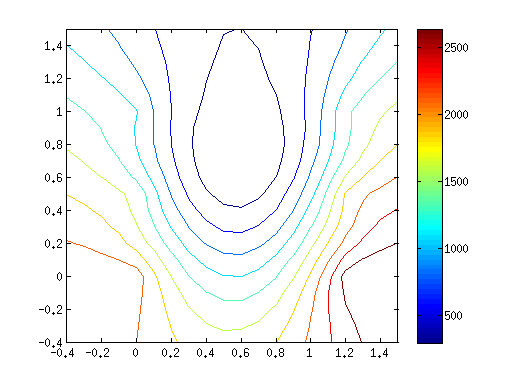
\includegraphics[width = 350pt]{nls_good.png}
  \caption{NLS loss function for the first configuration.}
  \label{nls_good}
  \end{center}
\end{figure}

\begin{figure}[H]
\begin{center}
  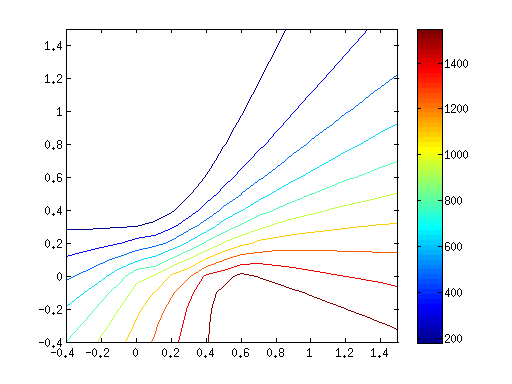
\includegraphics[width = 350pt]{nls_bad.png}
  \caption{NLS loss function for the second configuration.}
  \label{nls_bad}
  \end{center}
\end{figure}

\begin{figure}[H]
\begin{center}
  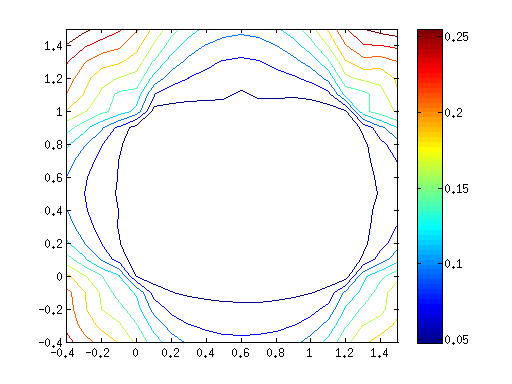
\includegraphics[width = 350pt]{crlb_good.png}
  \caption{Cramer-Rao lower bound for the first configuration.}
  \label{crlb_good}
  \end{center}
\end{figure}

\begin{figure}[H]
\begin{center}
  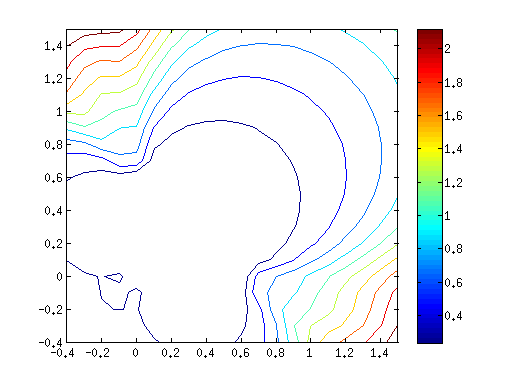
\includegraphics[width = 350pt]{crlb_bad.png}
  \caption{Cramer-Rao lower bound for the second configuration.}
  \label{crlb_bad}
  \end{center}
\end{figure}



\newpage
\section{Localisation}
\label{Localisationg}

\subsection{NLS using Gauss-Newton}
\label{lacalisation Gauss}
To compute the estimate target position for each time instant, the non-linear least square model with the Gauss-Newton algorithm is used here. The matlab code to compute the estimates is given below.
\begin{verbatim}
tphat = tphat;
for i = 1:length(y.y)-1
    y_k = sig(tphat(i,:),FS);
    xhat = nls(sm, y_k, 'thmask',zeros(1,sm.nn(4)));
    disp(i)
    est_target_pos(:,i)=xhat.x0(1:2);
    sm.x0=[xhat.x0(1:2); xhat.x0(3)+bias];
    display(xhat.x0)
end
SFlabCompEstimGroundTruth(est_target_pos, sensor_position');
\end{verbatim}
Using the time measurements and initial values contained in the sensor model, we can produce the output shown in the figure below.
\begin{figure}[H]
  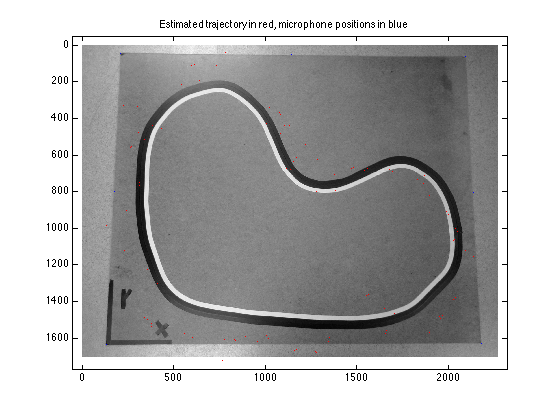
\includegraphics[width = 350pt]{NLS_target_est.png}
  \caption{NLS target estimation using Gauss-Newton}
  \label{NLS_target_est}
\end{figure}



\newpage
\subsection{TDOA approach}
\label{Pairwise difference approach}
By setting up a matrix with the pairwise differences of the sensor measurements for all time instances, the ''TDOA2'' sensor model can be used to estimate the target position. To do so the measurements must be described as a ''sig'' object. This whole process is shown below for one time instance $m$.
\begin{verbatim}
    yy = [];
    for k = 1:6,
        for l = k+1:7,
            yy = [yy tphat(m, k) - tphat(m,l)];
        end
    end
\end{verbatim}
 Then using a NLS-algorithm the target position for each time instant $m$ can be estimated. This can be achieved with the following code in matlab, which yields the figures below.
 \begin{verbatim}
    [shat, xhat] = nls(sm,sig(yy), 'thmask', zeros(sm.nn(4) ,1));
    sig_yy = sig(yy);
    x(:,m) = shat.x0;
    x_cov(:,:,m) = cov(shat.px0);
    sm.x0 = shat.x0;
    plot(shat, 'conf', 90)
 \end{verbatim}
 \begin{figure}[H]
   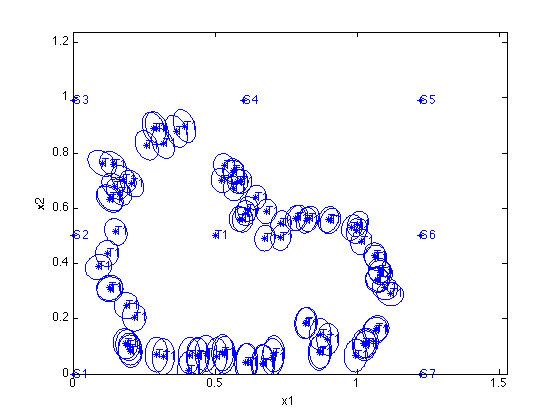
\includegraphics[width = 350pt]{TDAO_target_est1.png}
   \caption{Pairwise measurement differences using TDOA2 showing confidence interval}
   \label{TDOA_target_est1}
 \end{figure}
 \begin{figure}[H]
   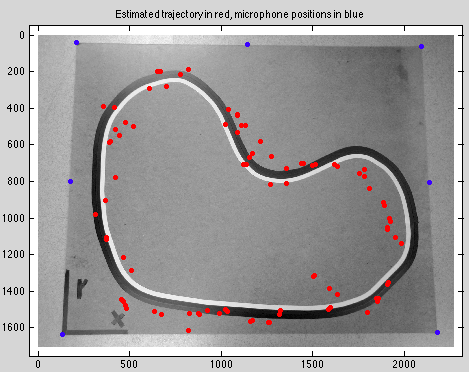
\includegraphics[width = 350pt]{TDAO_target_est2.png}
   \caption{Pairwise measurement differences using TDOA2}
   \label{TDOA_target_est2}
 \end{figure}
Figure \ref{TDOA_target_est2} compared to figure \ref{NLS_target_est} yields that the TDOA method with the pairwise differences gives a better estimate of the target positions. 


\newpage
\section{Tracking}
\label{Tracking}

\newpage
\section{Sensitivity analysis}
\label{Sensitivity analysis}

\newpage
\section{Conclusion}
\label{Conclusion}

\chapter{Appendix}
% .m code

\end{document}



%%% Local Variables: 
%%% TeX-PDF-mode: t 
%%% TeX-master: "rapport"
%%% End: 

